\documentclass[12pt]{article}
\usepackage[T1]{fontenc}
\usepackage[latin9]{inputenc}
\usepackage{textcomp}
\usepackage{amstext}
\usepackage{graphicx}
\usepackage{amssymb}
\makeatletter
\providecommand{\tabularnewline}{\\}

\usepackage{fourier-orns}
\usepackage[colorlinks,linkcolor=blue]{hyperref}

\usepackage{subfigure}
\usepackage{float}

\textwidth=6in
\topmargin=-1in
\oddsidemargin = -0.5in
\parindent=0.0cm
\parskip=0.3cm
\textwidth=7.5in
\textheight= 20in

\sloppy
\newtheorem{theorem}{Theorem}[section]
\newtheorem{lemma}{Lemma}[section]
\newtheorem{corollary}{Corollary}[section]
\newtheorem{definition}{Definition}[section]


\begin{document}
{\bf Part II: } 
\begin{figure}[H]
  \centering
  \setlength{\abovecaptionskip}{-0.1in}
  \setlength{\belowcaptionskip}{-0.15in}
	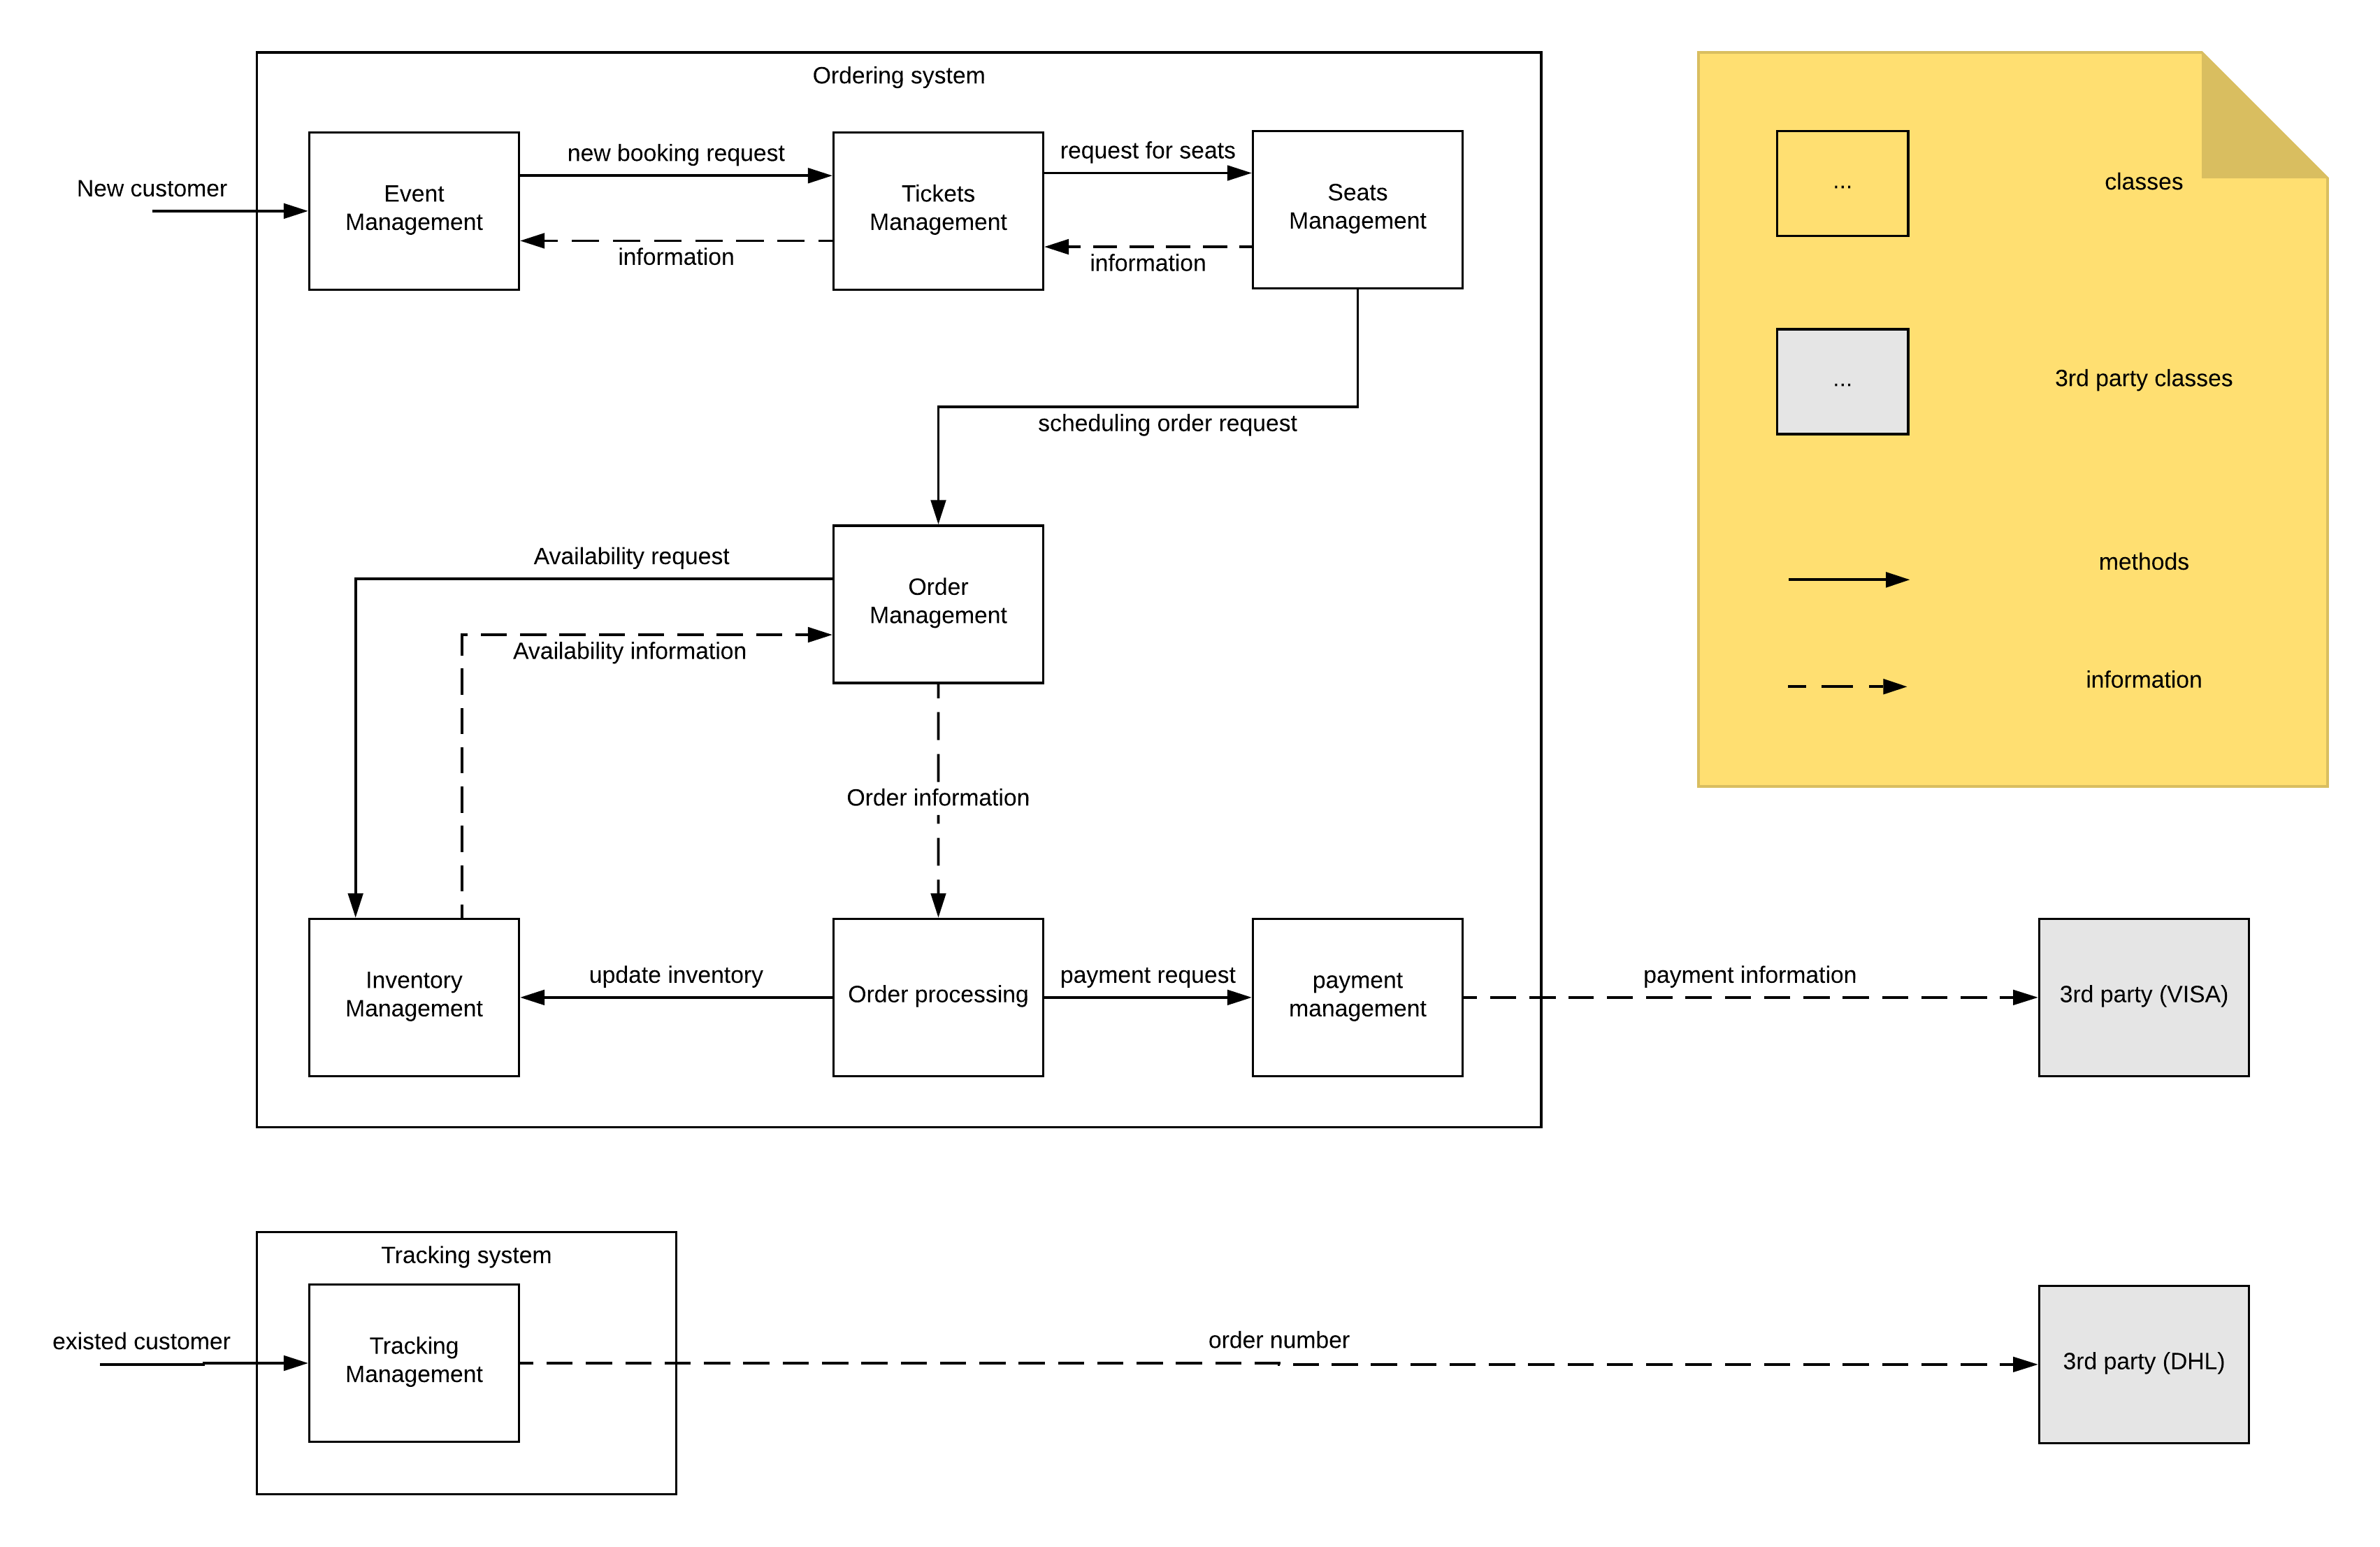
\includegraphics[width=0.8\linewidth]{topic_2.png}
	\caption{Functional view for ticket booking ststem}
\end{figure}
\begin{figure}[H]
  \centering
  \setlength{\abovecaptionskip}{-0.1in}
  \setlength{\belowcaptionskip}{-0.15in}
	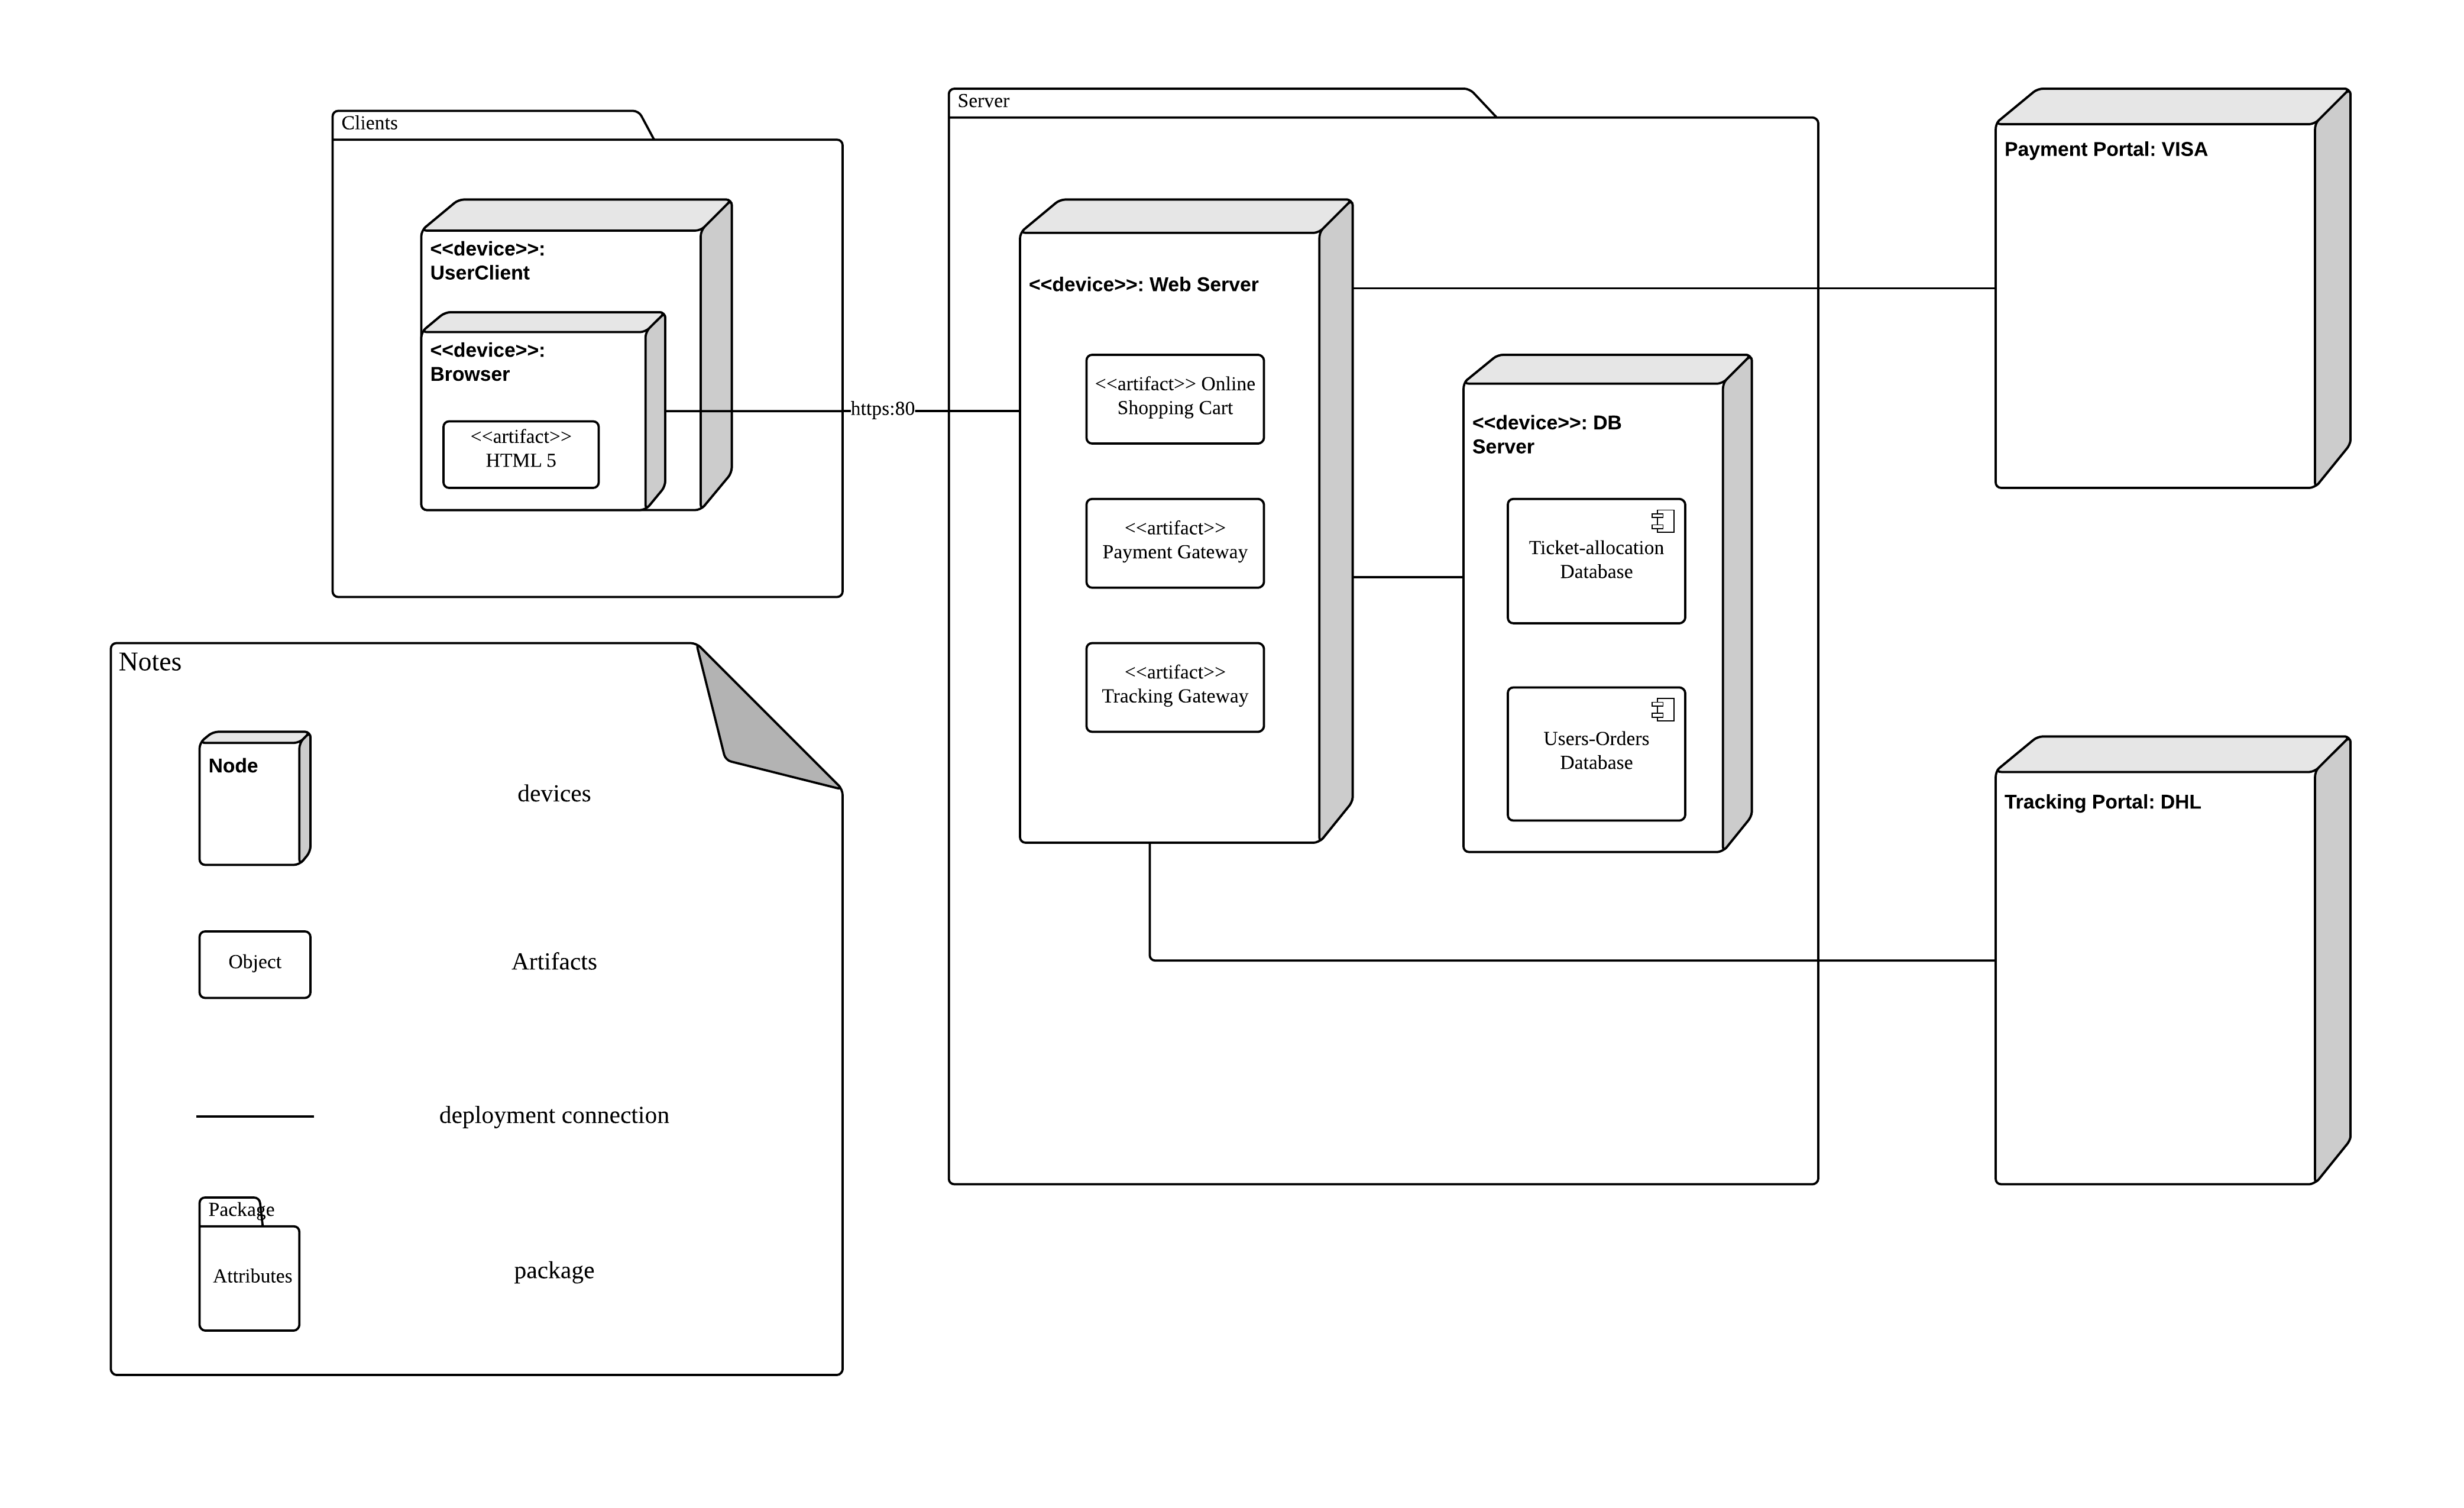
\includegraphics[width=0.8\linewidth]{deploy.png}
	\caption{Deployment view for ticket booking ststem}
\end{figure}
Figure 1 shows interaction between internal components. Its main target audience are new customers who have few professional knowledges in computing.\\
Figure 2 illustrates deployment for different devices. Its main target audience are software developers, such as front-end developers, database developers, network engineers, product managers. 
% Figure 1 shows a functional diagram of a online tickets booking/tracking system for the Royal Albert Hall. It aims at stakeholders who have few professional knowledges in computing, such as customers or users.\\[10px]
% New users can search for events they interested through the \texttt{EventManagement} module. When they intend to book a ticket for a particular event, a booking request is sent from \texttt{EventManagement} to \texttt{TicketManagement} (which will also send back proper success/error messages). 
% Afterwards, \texttt{TicketManagement} issues a seat request to the \texttt{SeatingManagement}. Secondly, \texttt{SeatingManagement} schedules an order request to \texttt{OrderManagement}. Meanwhile, \texttt{OrderManagement} requests to check availability for the requested event with \texttt{InventoryManagement} based on order information. 
% If it is available, \texttt{OrderManagement} sends the order information to the \texttt{OrderProcessing} module, which sents a payment request to \texttt{PaymentManagement}. 
% At the same time, the \texttt{OrderProcessing} module asks \texttt{InventoryManagement} to update the allocation state for the event. Finally, the \texttt{PaymentManagement} module can allow users to be redirected to a third party (e.g. VISA) to complete the payment by exchanging payment information. At this point, new customers complete the entire process of online tickets booking. \\[10px]
% For existing users, who has successfully made orders, they can directly send a request to view the delivering information. They will be redirected to to a third-party system (e.g. DHL) by the \texttt{TrackingManagement} module to track their deliveries.

\end{document}